\documentclass[a4paper]{article}

\usepackage{tecnico_relatorio}


\usepackage[hypcap]{caption} % makes \ref point to top of figures and tables
\usepackage{rotating}
\usepackage{multirow}
\usepackage{indentfirst} % indent first paragraph in section
\usepackage{geometry}
\usepackage{fancyvrb}

\begin{document}
	\trSetImage{img/tecnico_logo}{6cm} % Logotipo do Técnico
	\trSetSubject{Arquitecturas Avançadas de Computadores}
	\trSetType{Laboratório III}
        \trSetTitle{Paralelização e Aceleração de um Algoritmo}

	
	\trSetBoxStyle{0.3}
	
	\trSetAuthorNr{3}
	
	\trSetAuthors
	{
		\begin{center}
			Gonçalo Ribeiro

			73294
		\end{center}
	}{
		\begin{center}
			Miguel Costa

			73359
		\end{center}
	}{
		\begin{center}
			Rafael Gonçalves

			73786
		\end{center}
	}
		
	\trSetProfessor{Prof. Leonel Sousa}
	
	\trMakeCover
	
	\tableofcontents
	\pagenumbering{gobble}
	\pagebreak
	\pagenumbering{arabic}
	\setcounter{page}{1}
	
	\section{\textit{Abstract}}
	
	A paralelização e aceleração de um programa é algo fundamental no que toca ao desenvolvimento de algoritmos de computação. O aumento constante na quantidade de informação e dados faz com que tenha que haver uma preocupação na descodificação e computação desses mesmos dados de forma a que seja possível a obtenção de resultados em tempo útil. Desta forma, a computação paralela e aceleração de um programa é cada vez mais um problema com mais interesse e utilidade. Esta aceleração pode ser feita de diversas maneiras, sendo que aqui se procura a utilização de instruções de processamento vectorial para consegui-la, aplicadas a uma função de \textit{smoothing} para a obtenção de um sinal filtrado do seu ruído, possivelmente resultante da amostragem de sinal.
	
	
	\section{Introdução}
	
	O objectivo do presente trabalho laboratorial é a aceleração e paraleliazação de um algoritmo de \textit{smoothing}. Foi dada a possibilidade de realizar este projecto recorrendo a instruções vectoriais ou utilizando uma unidade de processamento gráfico (GPU), sendo que se escolheu utilizar instruções vectoriais suportadas pela arquitectura Intel IA32e (MMX, SSEx, AVX).
	
	O algoritmo de \textit{smoothing} consiste na obtenção de uma função aproximada, em que é filtrado todo o ruído resultante da amostragem do sinal. Na \autoref{fig:fun_smoothing} estão representados dois gráficos, em que o primeiro demostra o sinal com ruído e o segundo a função resultante após se aplicar a função de \textit{smoothing}.
	
		\begin{figure}[h]
			\centering
			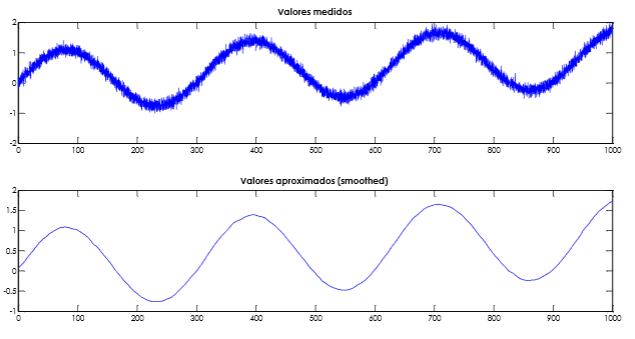
\includegraphics[width=1.\textwidth]{img/fun_smoothing}
			\caption{Resultado da aplicação de \textit{smoothing} a um sinal com ruído. }
			\label{fig:fun_smoothing}
		\end{figure}
		
	Para calcular o \textit{smoothing} foi fornecida a equação que permite calcular os valores aproximados $\hat{y}_1,\ ...\ , \hat{y}_{N-1}$, a partir da função original, com domínio $x_1,\ ...\ ,x_{N-1}$, e pontos (afectados de ruído) $y_1,\ ...\ , y_{N-1}$:
	
	\begin{equation}
		\hat{y}_i =  \frac{ \sum_{k=0}^{N-1} K_b (x_i, x_k ) y_k}{\sum_{k=0}^{N-1} K_b (x_i, x_k )} 
		\label{eq:smoothing_function}
	\end{equation}
	
	onde
	
	\begin{equation}
		K_b (x_i,x_k)=exp\left(-\frac{(x-x_k)^2}{2b^2} \right)
		\label{eq:smoothing_kb}
	\end{equation}
	 	
	 	 
	Também é já fornecido no enunciado um algoritmo (Algoritmo 1) que ilustra um exemplo para calcular o resultado da função de \textit{smoothing}.
	
	
	\section{Aceleração e Paralelização}
	\label{sec:implementations}
	
	Para realizar a aceleração do programa foram adoptadas várias estratégias: usando instruções de processamento vectorial de 128 bits e usando instruções de processamento vectorial de 128 bits com \textit{unrolling} do ciclo de computação em 2, 3, 4 e 8 cálculos por ciclo.
	
	A primeira tarefa a executar é então alocar a memória necessária para os dados e para os resultados. Para tal usou-se uma função já fornecida pelo professor (\texttt{aligned\_malloc()}) que permite alocar um tamanho desejado de memória, com a particularidade de que é garantido que esta memória está alinhada na memória. Tal não é garantido pela função \texttt{malloc()} e para o uso das instruções vectoriais é imprescindível que os dados a processar estejam alinhados.
	
	De seguida são corridas as funções em teste. Os resultados de todas as soluções com instruções vectoriais são comparadas com uma função escrita directamente com base no Algoritmo 1 do enunciado, a que se chamou \texttt{normal\_smoothing()}:
	
	\begin{verbatim}
void normal_smoothing(float *x, float *y, float *res, int len) {
    int i,j;
    float sumA, sumB, factor;
    
    for(i=0; i<len; i++){
        sumA = sumB = 0;
        for(j=0; j<len; j++){
            factor = exp((-(x[i]-x[j])*(x[i]-x[j]))/(2*_SMOOTH*_SMOOTH));
            sumA += factor*y[j];
            sumB += factor;
        }
        res[i] = sumA/sumB;
    }
}
	\end{verbatim}
	
	
	Antes de se medir qualquer tempo, o algoritmo em análise é corrido uma vez, de modo a tentar que as instruções e dados estejam em \textit{cache}. Isto é feito tanto para as soluções com instruções vectoriais como para a função \texttt{normal\_smoothing()}.
		
	Após se obterem os diversos valores temporais, é liberta a memória anteriormente alocada e são verificados os resultados do \textit{smoothing} obtidos de modo a comprovar se se chegou ao resultado desejado: remover o ruído do sinal original.
	
	\subsection{\texttt{smoothing\_simple()}}
	
	Esta função implementa o algoritmo de \textit{smoothing} recorrendo a instruções vectoriais. O ciclo interno é paralelizado visto que cada operação é feita sobre 4 ou 8 dados em simultâneo (conforme se esteja a usar a versão de 128 bits ou a de 256).
	
	Uma optimização que foi feita foi fazer uma única divisão por cada chamada da função: embora a função de \textit{smoothing} contenha uma divisão que é feita $i \times j$ vezes o divisor é constante, pelo que a optimização utilizada consiste em calcular o inverso do divisor uma única vez e a partir desse momento usar sempre multiplicações. Isto resulta numa optimização porque segundo Intrinsics Guide da Intel as divisões com instruções vectoriais demoram mais ciclos do que as multiplicações.
	
	Como exemplo apresenta-se a função \texttt{sse128\_smoothing\_simple()}, que consiste na implementação da \texttt{smoothing\_simple()} para instruções vectoriais de 128 bits. Para alocar o vector \texttt{aux} usou-se a \texttt{aligned\_malloc()} visto que a função \texttt{\_mm\_store\_ps()} escreve para uma posição alinhada de memória.
	
	\begin{verbatim}
void sse128_smoothing_simple(float *x, float *y, float *res, int len) {
    float *xi, *xj, *yj;
    float *aux = (float*) aligned_malloc(4*sizeof(float));
    float sumAtot, sumBtot;

    __m128 sumA, sumB;
    __m128 divisor = _mm_div_ps(_mm_set_ps1(1.0), _mm_set_ps1(2*_SMOOTH*_SMOOTH));
    __m128 exponential;
    __m128 cache;

    for(xi=x; xi < x+len; xi++, res++)
    {
        sumA = sumB = _mm_setzero_ps();

        for(xj=x, yj=y; xj < x+len; xj+=4, yj+=4)
        {
            // e^[(-(xi-xj)^2) / (2*smoothing^2)]
            cache = _mm_sub_ps(_mm_load_ps1(xi), _mm_load_ps(xj));
            
            exponential = _mm_exp_ps(
                    _mm_mul_ps(
                        _mm_sub_ps(_mm_setzero_ps(),
                            _mm_mul_ps(
                                cache,
                                cache
                                )), divisor));

            sumB = _mm_add_ps(sumB, exponential);
            sumA = _mm_add_ps(sumA, _mm_mul_ps(_mm_load_ps(yj), exponential));
        }

        // horizontaly add sumA and sumB
        _mm_store_ps(aux, _mm_hadd_ps(_mm_hadd_ps(sumA, sumB), _mm_setzero_ps()));

        sumAtot = aux[0];
        sumBtot = aux[1];

        *res = sumAtot/sumBtot;
    }

    aligned_free(aux);
}
	\end{verbatim}		

	
	\subsection{\texttt{smoothing\_unroll*()}}
	\label{subsec:implementation_unrolling}
	
	Para tentar conseguir uma aceleração superior à conseguida com \texttt{smoothing\_simple()} foram implementadas versões que usam \textit{unrolling} do ciclo interno. Foram testados 4 casos de \textit{unrolling}: 2, 3, 4 e 8 instruções por ciclo, sendo que como se pode constatar pela \autoref{tab:results_128} teve-se sucesso em aumentar o \textit{speedup}.
	
	O \textit{unrolling} máximo que é possível é limitado pelo número de registos disponíveis. Tendo em conta que o processador usado (i7-3820) é um processador de 64 bits e que suporta AVX, deverão existir 16 registos vectorias (YMM0 -- YMM15). Calcula-se que com \textit{unrolling} de 4 todos os registos já estariam utilizados, pelo que se esperava que com \textit{unrolling} de 8 os resultados fossem piores do que com 4. Pela \autoref{tab:results_128} ao contrário do esperado o \textit{unrolling} de 8 conseguiu ainda ser superior ao de 4, se bem que apenas em 2\% no máximo. Para explicar este fenómeno deveria ser analisado o \textit{assembly} produzido para verificar a utilização dos registos. É possível também que este comportamento se deve a efeitos introduzidos pela cache.
	
	
	\section{Resultados} 
	
	Para comparar os resultados das várias soluções foram calculados \textit{speedups} que usam como base de comparação os resultados da função \texttt{sse128\_smoothing\_simple()}, descrita em \ref{sec:implementations}. Nas tabelas de resultados a coluna ``vector length" refere-se ao número de amostras da função sobre a qual se está a fazer o \textit{smoothing}. A coluna ``original time" representa o tempo que a função \texttt{smoothing\_normal()} demorou a ser executada.
	
	Para instruções vectoriais de 128 bits o \textit{speedup} teórico é de 4 vezes, visto que são feitas operações sobre quatro \texttt{float}s de cada vez, em vez de apenas um. Como se pode verificar pela \autoref{tab:results_128} com a solução simples conseguiu-se um \textit{speedup} de cerca de 3.1 vezes, que representa 77\% do máximo teórico. Com \textit{unrolling} de 2 conseguiu-se ficar a 92\% do valor máximo e com \textit{unrolling} de 4 atingiu-se 99\% desse valor. Para \textit{unrolling} de 8 previa-se uma queda de desempenho (como explicado em \ref{subsec:implementation_unrolling}), o que não aconteceu, tendo-se mesmo passado o \textit{speedup} teórico máximo em consistentemente em vários testes.
	
	Nota-se que para dados com tamanho 128 e 256 existem vários \textit{speedups} que ultrapassam 4, chegando alguns a 10. Isto é explicado por efeitos introduzidos pela \textit{cache}.
	

	\begin{table}[h]
	\caption{Resultados para extensões multimédia de 128 bits}
	\label{tab:results_128}
	\begin{Verbatim}[fontsize=\small,xleftmargin=-3mm]
=============================================================================================
   COMPUTING SMOOTHING SPEEDUP for SSE-128
=============================================================================================
| Vector |   Original |   speedup   |   speedup   |   speedup   |   speedup   |   speedup   |
| Length |  Time [us] |    simple   | unrolling 2 | unrolling 3 | unrolling 4 | unrolling 8 |
+--------+------------+-------------+-------------+-------------+-------------+-------------+
|     16 |        4.6 |    0.884615 |    0.958333 |    0.410714 |    0.920000 |    0.171642 |
|     32 |       61.2 |    3.090909 |    3.600000 |    4.935484 |    5.563636 |    4.309859 |
|     64 |      237.4 |    2.799528 |    3.618902 |    2.580435 |    3.450581 |    3.440580 |
|    128 |      929.4 |    3.812141 |   10.707373 |   10.146288 |    4.732179 |    4.302778 |
|    256 |     2006.2 |    4.965842 |    5.876391 |    5.591416 |    6.393244 |    5.499452 |
|    512 |     4689.4 |    3.082698 |    3.663021 |    3.795241 |    3.982167 |    3.940010 |
|   1024 |    21119.0 |    2.736969 |    3.145236 |    3.231478 |    3.362470 |    3.361292 |
|   2048 |    93695.2 |    2.919054 |    3.363386 |    3.491712 |    3.595585 |    3.606880 |
|   4096 |   408000.6 |    3.171430 |    3.693677 |    3.836525 |    3.947367 |    3.982164 |
|   8192 |  1634784.8 |    3.165204 |    3.724790 |    3.882026 |    3.964539 |    4.029549 |
|  16384 |  6482300.2 |    3.153480 |    3.720566 |    3.879947 |    3.960604 |    4.033608 |
|  32768 | 25781057.0 |    3.144238 |    3.711833 |    3.877029 |    3.953504 |    4.032080 |
+--------+------------+-------------+-------------+-------------+-------------+-------------+
	\end{Verbatim}
	\end{table}


	Na \autoref{tab:results_256} apresentam-se os resultados obtidos quando usadas instruções vectoriais de 256 bits. 

        Estes resultados parecem surpreendentemente baixos face ao esperado. Como tal, foi utilizado o GNU Debugger (\texttt{gdb}) para fazer o \textit{disassemble} do programa, de maneira a tentar descobrir operações responsáveis pela quebra de performance. Esta investigação, porém, não levou a conclusões viáveis.
	
	
	\begin{table}[h]
	\caption{Resultados para extensões multimédia de 256 bits}
	\label{tab:results_256}
	\begin{Verbatim}[fontsize=\small,xleftmargin=-3mm]
=============================================================================================
   COMPUTING SMOOTHING SPEEDUP for SSE-256
=============================================================================================
| Vector |   Original |   speedup   |   speedup   |   speedup   |   speedup   |   speedup   |
| Length |  Time [us] |    simple   | unrolling 2 | unrolling 3 | unrolling 4 | unrolling 8 |
+--------+------------+-------------+-------------+-------------+-------------+-------------+
|     16 |        4.6 |    0.489362 |    0.500000 |    0.264368 |    0.230000 |    0.131429 |
|     32 |       62.0 |    2.279412 |    2.605042 |    1.890244 |    2.924528 |    1.319149 |
|     64 |      233.0 |    2.971939 |    3.509036 |    2.807229 |    3.290960 |    3.319088 |
|    128 |      439.4 |    5.604592 |    5.890080 |    3.736395 |    4.605870 |    4.359127 |
|    256 |     2103.6 |    7.412262 |    8.448193 |    7.980273 |    8.475423 |    8.294953 |
|    512 |     4683.6 |    4.677986 |    5.040465 |    4.554259 |    5.021012 |    4.941549 |
|   1024 |    21110.8 |    2.220740 |    2.307797 |    2.268369 |    2.323238 |    2.320021 |
|   2048 |    93581.2 |    2.080155 |    2.168701 |    2.153688 |    2.198207 |    2.187356 |
|   4096 |   407518.2 |    2.163882 |    2.269379 |    2.283686 |    2.309500 |    2.280649 |
|   8192 |  1634150.0 |    2.135391 |    2.252925 |    2.278696 |    2.305896 |    2.272658 |
+--------+------------+-------------+-------------+-------------+-------------+-------------+
	\end{Verbatim}
	\end{table}

	
	\section{Dificuldades}
	
	 Aquando da demonstração, os resultados de \textit{speedup} obtidos eram muito inferiores ao esperado (estando-se a obter valores de speedup próximos de 1). Contudo, após uma análise mais detalhada sobre o funcionamento de instruções vectoriais, verificou-se que, apesar da não se estar a usar a porção de código correspondente ao uso de instruções de processamento vectorial para 256 bits, o facto de existir esta porção de código fazia com que o compilador agendasse mudanças de modo entre o processamento de 128 bits e o de 256 bits, o que atrasava imenso a execução do programa. Como tal separam-se estas duas componentes de processamento em dois programas distintos. Esta simples mudança fez com que, ao usar as instruções de processamento de 128 bits, se conseguisse atingir resultados de \textit{speedup} compatíveis com os esperados. Num site sobre programação de xadrez\footnote{\url{https://chessprogramming.wikispaces.com/AVX}} encontrou-se a seguinte referência a este problema:
	 
	 \begin{quote}
	  ``Intel strongly advises against mixing SSE 128-bit instructions and AVX 256-bit instructions, as this ``mode-switching'' can cost upwards of 70 clock cycles. However, mixing SSE 128-bit and AVX 128-bit is okay, as is mixing AVX 128-bit and AVX 256-bit.''
	 \end{quote}
	   

	
	\section{Conclusão}

	Com esta actividade experimental o grupo conseguiu cumprir o objectivo de acelerar o programa proposto. Através da utilização de instruções de processamento vectorial conseguiu-se filtrar todo o ruído de um sinal, obtendo-se uma função aproximada deste mesmo sinal (\textit{smoothing}).
	
	Para tal, foi desenvolvida a utilização de instruções de 128 e 256 bits, sendo que se adoptaram várias estratégias para conseguir esta aceleração sobre o programa original. Os resultados obtidos para a versão de 128 bits encontram-se dentro do esperado (\textit{speedup} próximo de 4), mas, para a versão de 256 bits, os resultados encontram-se aquém do antecipado (apenas se conseguindo uma aceleração pouco superior a 2, longe dos \textit{speedups} de 8 previstos).
	
	Em suma, o grupo conseguiu pôr em prática alguns conceitos acerca da paralelização e aceleração de um programa.


\end{document}
